\documentclass[table]{book}


\usepackage[width=6.5in, height=9.0in, top=1.0in, papersize={8.5in,11in}]{geometry}
\usepackage[pdftex]{graphicx}
\DeclareGraphicsExtensions{.pdf,.png,.jpg}
%\usepackage{draftwatermark}
\usepackage{amsmath}
\usepackage{amsthm}
\usepackage{amssymb}
%\usepackage{txfonts}
\usepackage{textcomp}
%\usepackage{amsthm}
%\usepackage{array}
%\usepackage{datetime}
\usepackage{anyfontsize}
\usepackage{t1enc}
\usepackage[section,subsection]{extraplaceins}   %%%  \FloatBarrier
\usepackage[all]{xy}
\usepackage{fancyhdr}
\usepackage{hyperref}
\usepackage{verbatim}
\usepackage{algorithm}
\usepackage{algorithmic}
\usepackage{makeidx}
\usepackage{multicol}
\usepackage{multirow}
\usepackage{color}
\usepackage{rotating}
\usepackage{wrapfig}
%\usepackage{tabularx}
\usepackage{xcolor}
\usepackage{framed}
\usepackage{xspace}
\usepackage{listings}
\lstset{language=python,frame=ltrb,framesep=5pt,basicstyle=\normalsize,
 keywordstyle=\ttfamily\color{DarkRed},
%morecomment=[n][\textbf]{In\ [}{]\:},
%morecomment=[n][\textbf]{Out\ [}{]\:},
morecomment=[s][\color{blue}]{In\ [}{]\:},
morecomment=[s][\color{red}]{Out[}{]\:},
identifierstyle=\ttfamily\color{DarkBlue}\bfseries,
commentstyle=\color{OliveGreen},
stringstyle=\ttfamily,
showstringspaces=false,tabsize = 3}

\lstdefinelanguage{shell} {
commentstyle = \color{black},
keywordstyle = \color{black},
stringstyle = \color{black},
identifierstyle = \color{black},
morecomment=[s][\color{blue}]{In\ [}{]\:},
morecomment=[s][\color{red}]{Out[}{]\:},
 }

\newtheorem{thrm}{Theorem}
\newtheorem{lem}[thrm]{Lemma}
\newtheorem{cor}[thrm]{Corollary}
\newtheorem{rem}[thrm]{Remark}
\newtheorem{defn}[thrm]{Definition}
\newtheorem{exmpl}[thrm]{Example}

% this gives a little box for the end of a proof:
%
\def\endthrmbox{$\sqsubset \!\!\!\! \sqsupset$}

\newcommand{\dis}{\displaystyle}
 \def      \RR             {{\mathbb R}} 
        \def      \NN             {{\Bbb N}} 
        \def      \QQ             {{\Bbb Q}} 
        \def      \CC             {{\Bbb C}} 
        \def      \ZZ             {{\Bbb Z}} 
 
 
        \def       \a              {{\alpha}} 
        \def       \b              {{\beta}} 
        \def       \d              {{\delta}} 
        \def       \D              {{\Delta}} 
        \def         \e              {{\varepsilon}} 
        \def         \g              {{\gamma}} 
        \def         \G              {{\Gamma}} 
        \def       \l              {{\lambda}} 
        \def       \L              {{\Lambda}} 
        \def        \m               {{\mu}} 
        \def         \n              {{\nabla}} 
        \def       \var          {{\varphi}} 
        \def         \s              {{\sigma}} 
        \def       \Sig          {{\Sigma}} 
        \def       \Om          {{\Omega}} 
 
        \def       \t              {{\tau}} 
        \def         \th             {{\theta}} 
        \def       \O              {{\Omega}} 
        \def       \o              {{\omega}} 
        \def         \z              {{\zeta}} 
       \def        \P             {{\Phi}} 
       \def        \p             {{\phi}} 
        %Other macros 
 
        \def       \iy              {{\infty}} 
        \def         \pa             {{\partial}} 
        \def         \div           {{\rm div}} 
         \def       \na            {{\nabla}} 
 



\newcommand{\pythonlogo}{
\\[-2mm] \begin{picture}(0,0)
\put(-40,-40){\includegraphics[scale=0.25]{./Figures/pythonlogo.png}}
\end{picture}
}

\newcommand{\clogo}{
\\[-2mm] \begin{picture}(0,0)
\put(-30,-30){\includegraphics[scale=0.2]{./Figures/clogo.png}}
\end{picture}
}

\newcommand{\roslogo}{
\\[-2mm] 
\begin{picture}(0,0)
\put(-30,-30){\includegraphics[scale=0.2]{./Figures/roslogo.png}}
\end{picture}
}

\newtheorem{summary}{Summary:}
\newtheorem{example}{Example:}[section]

\definecolor{OliveGreen}{cmyk}{0.64,0,0.95,0.40}
\definecolor{DarkBlue}{cmyk}{0.76,0.76,0,0.20}
\definecolor{DarkRed}{cmyk}{0,1,1,0.45}


\def      \RR             {{\mathbb R}} 
\def      \DS            {\displaystyle} 

\setlength{\oddsidemargin}{0mm} 
\setlength{\evensidemargin}{0mm} 

%\SetWatermarkLightness{0.975}
%\SetWatermarkScale{6}
%\SetWatermarkText{\includegraphics{test.png}}

\pagestyle{fancy}
\renewcommand{\chaptermark}[1]{\markboth{#1}{}}
\renewcommand{\sectionmark}[1]{\markright{\thesection\ #1}}
\fancyhf{}
\fancyhead[LE,RO]{\bfseries\thepage}
\fancyhead[LO]{\bfseries\rightmark}
\fancyhead[RE]{\bfseries\leftmark}
\renewcommand{\headrulewidth}{0.5pt}
\renewcommand{\footrulewidth}{0pt}
\addtolength{\headheight}{0.5pt}
\setlength{\footskip}{0in}
\renewcommand{\footruleskip}{0pt}
\fancypagestyle{plain}{%
\fancyhead{}
\renewcommand{\headrulewidth}{0pt}
}


\definecolor{color02}{rgb}{0.18,0.35,0.59}
\definecolor{color03}{rgb}{0.44,0.59,0.82}
\definecolor{color06}{rgb}{0.35,0.35,0.35}


\definecolor{MSBlue}{rgb}{.204,.353,.541}
\definecolor{MSLightBlue}{rgb}{.31,.506,.741}
\definecolor{MSBlue1}{rgb}{0.18,0.35,0.59}
\definecolor{MSBlue2}{rgb}{0.44,0.59,0.82}
\definecolor{MSBlue3}{rgb}{0.35,0.35,0.35}

\usepackage{titlesec}
\titleformat{\chapter}[display]
%{\normalfont\bfseries\color{MSBlue1}}    %\normalfont\bfseries\filcenter}
{\normalfont\bfseries}    %\normalfont\bfseries\filcenter}
{\LARGE\thechapter}
{1ex}
{\titlerule[2pt]
\vspace{2ex}%
\LARGE}
[\vspace{1ex}%
{\titlerule[2pt]}]



\date{\today}



\title{{\rule{\linewidth}{0.5mm}}\\[2mm]{\huge\bfseries Final Project}\\[-1mm]{\rule{\linewidth}{0.5mm}} \\  \vfill
{\LARGE \bfseries Natural Computing Homework}\vfill}
\author{Paul Blasi \and Jaysen Spurlock}
\date{\today}


\begin{document}

\frontmatter

\addcontentsline{toc}{chapter}{Title}
\maketitle
\tableofcontents
\addcontentsline{toc}{chapter}{Contents}
%\listoffigures
%\addcontentsline{toc}{chapter}{List of Figures}

\chapter{Document Preparation and Updates}
% !TEX root = FinalProject.tex

Current Version [0.0.1]
\vspace*{5mm}

{\color{MSBlue3}
\noindent
\textit{Prepared By:}\\
\textit{Jaysen Spurlock}\\
\textit{Paul Blasi}
}

\newcommand{\revision}[4]
{
    \textit{\textbf{#1}}
    & \textit{\textbf{#2}}
    & \textit{\textbf{#3}}
    & \textit{\textbf{#4}}
    \tabularnewline\hline
}

\vfill
\noindent
{\color{color02} \textit{\textbf{Revision History}}}\\
\begin{tabular}{|>{\raggedright}p{1.5cm}
                |>{\raggedright}p{3cm}
                |>{\raggedright}p{1.5cm}
                |>{\raggedright}p{9cm}
                |}
\hline

\revision{Date}{Author}{Version}{Comments}
\revision{5/6/15}{Jaysen Spurlock}{0.0.0}{Initial document creation}
\revision{5/6/15}{Jaysen Spurlock}{0.0.1}{Filled out problem statement}
\end{tabular}
\vfill


\mainmatter

% ~~~~~

% Complete problem statement
% !TEX root = FinalProject.tex

\chapter{Problem Statement}




% Background and literature review
% !TEX root = FinalProject.tex

\chapter{Background}




% Problem solution
% !TEX root = FinalProject.tex

\chapter{Solution}

\section{Phase 1 - Design Approach}
	% Talk about initial design of game system/rules
	% Mention client/server architecture, and decisions to develop
	%  server from algorithm to network, and
	%  client from GUI to algorithm to network.

When starting out on this project, all that we knew is that we wanted to make a
game based in Natural Computing. We realized very early that an evolutionary
algorithm would be essential to create dynamicism in the game and ensure it was not
a simple, repetitive program. However, an evolutionary algorithm alone would not be
quite enough. We played around with the idea of putting the animals on a grid, to
allow them to interact with one another and explore the area. \\
Fortunately, we had this realization at about the time that the class was covering
Ant Colonies. The idea of pheromones was quickly snatched up.

When the class covered Cellular Automata, we realized that what we were building
would work very well in this sort of architecture. Our ``CA" cheated a little;
rather than depending solely on neighboring positions and states, we look at
neighborhoods to find competitors and randomly decide what happens after that,
based on a simple rule set and the players' settings.

At about the same time, the idea of splitting the project into a client-server
architecture began to hold more promise. With this sort of design, we could
distribute the individual EAs amongst the clients, with each being responsible for
evolving its own creatures. The server, meanwhile, would poll their statistics and
run the grid simulation to determine whether any of the creatures had conflict.

Once we decided our architecture, we moved on to considering how to build the 
client and server. Since they were communicating over the network, they need not
use the same language. We discussed the possibilities at length, initially 
considering Python for everything, but worrying that it would not be quite fast
enough for the server's purpose. Thus, we decided that C++ would better suit the
server, since it had no graphical requirements and would need as much speed as it
could get. The client, however, would be better off with visuals, so Python is the
language we chose for that. (We did consider whether the EA would move quickly
enough; in the end, we decided that we would try, and convert to C++ later if need
be.) \\
With the basic design considerations in place, we broke up the work -- Jaysen
offered to build the server, and Paul was happy to work on the client.

Finally, before any actual development could begin, we needed to know what our
program would actually do. Paul already had many ideas for the program. The rules
would focus entirely on the low-level agents in the simulation: they would have
certain mentalities and abilities, and act randomly with weights based on their
attributes.
\begin{description}
    \item[Prey v. Predator] This mentality determines how likely an agent is to
        seek out locations that contain other species.
    \item[Group v. Lone] This mentality determines how likely an agent is to seek
        out locations that contain their own species.
    \item[Strength v. Speed] This ability determines which reaction an agent will
        give in conflict, and how likely they are to succeed with it.
    \item[Lifetime v. Reproduction] This attribute determines whether a species is
        more likely to live a longer time, or to produce more children.
    \item[Senses] This attribute determines how likely an agent is to see another
        agent on the grid.
\end{description}
Meanwhile, Jaysen had several ideas for the implementation of the game.
\begin{description}
    \item[Pheromones] An idea borrowed from Ant Colonies, pheromones would be used
        to track where agents had been in the grid. This would play in with the
        different mentalities involving movement based on other agents.
    \item[Roulette] An idea borrowed from Evolutionary Algorithms, a roulette
        selection would be the tool of choice for determining the results of
        conflicts. Each agent would be weighted accordingly, by their relevant
        attribute.
    \item[Grid Tracking] Directly used from Cellular Automata, the idea of tracking
        agents in a common grid is almost a necessity for neighborhood checking.
    \item[Agent Tracking] In addition to CA's mapping, we will use the idea of
        tracking individual agents from Particle Swarms. This will increase the
        memory space requirements for the program, but on a server model, speed is
        more important.
\end{description}

Thus, we were ready to begin constructing the project.

\section{Phase 2 - Prototype $\alpha$}
	% Talk about initial steps taken in design.
	% Server was a mish-mash of code to get a running ``CA''
	% Client was a sandbox GUI to figure out program structuring approach
Once the design had been sufficiently fleshed out, we began working on our 
respective project components. This initial prototype is simply an effort to get
our thoughts put into code on our algorithms, which will allow us to create a
better structure later on and help decide what is needed in network communication.

\subsection{The Server}
The initial phase of the server was simply algorithm creation. Jaysen implemented
a number of functions to initialize a set of variables, so that he would have some
sample data to run the program with.

\subsection{The Client}
The initial phase of the client was more a proof of concept for the UI. Tkinter is a very basic GUI creation library so we needed to make sure that all of the features we would need would be available.

With some simple GUI created, it was apparent that Tkinter would work fine for all of the input needed and navigating between all of the different pages we had in mind. The last issue was whether or not we would be able to create the map after receiving an update from the server.

This was the most worrisome component in using Tkinter. Tkinter is not meant for image manipulation and doesn't have the ability to open many file types so it was looking bad. A solution does exist without importing PIL though. Using the PhotoImage class in Tkinter you can manipulate individual pixels, which is exactly what we needed.

\section{Phase 2 - Prototype $\beta$}
	% Talk about next steps taken in design.
	% Server was modularized and broken down into classes
	% Client solified MVC pattern and developed algorithms
After the initial phase was finished, we went back into our code to clean things up
and create some modularity. This would allow us to address any issues that we
discovered with our now-running algorithms without having to delve through massive
functions.

\subsection{The Server}
Jaysen opted to break the functionality up by creating an ``Engine" class, which
encapsulates the algorithm and hides components that aren't needed in general.

\subsection{The Client}
Since we had a proof of concept with the UI, it was time to get our hands dirty with some Natural Computing. The client's job was to evolve the traits of the individual species so an Evolutionary Algorithm was needed.

This EA was more complex than previous ones done in the homework sets. For starters, it needed to have a variable population, and to make the gameplay work it needed to be a relatively stable population. This was done by choosing the number of children to create by making sure they would replace all of the individuals that had died from aging, and then adding a gaussian random number with a mean of 0 and a standard deviation relating to the species reproduction value.

The EA also had to have an adaptive fitness function, which was also interesting. We accomplished this by multiplying each individual's trait by the focus that a user put on that trait, then normalizing all of the fitness values to between 0 and 1. This simplistic model gives good results when the user wants to put focus on something, but when no focus is set, the children are created from the same individuals many generations in a row. to avoid this, a flag is set if no focus is given so that the individuals are chosen randomly from the list.

The last new experience for the team regarding the EA was the variable lifespan of the individuals. The original attempt at this had each individual's lifespan generated by its own lifespan value. This had the interesting effect of evolving a high lifespan value without any focus on the value. While interesting, this was not a desired outcome of the algorithm so we patched it by using the species' lifespan value instead of the individual's.

\section{Phase 3 - Networking Structure}
	% Discuss networking structure (agreed-upon transmission protocol)
Once the algorithms had been implemented and we understood exactly what we needed
from the other application, it was easy enough to construct a protocol for message
passing over the network. The basic format of a message is as follows.

[1-byte message type] [4-byte message length, N] [N-byte message]

Message type may be one of the following.
\begin{description}
    \item[READY (0)] The message relates to the readiness of a client to begin.
    \item[PLAYER\_UPDATE (1)] The message relates to an update in the player list.
    \item[INDEX (2)] The message relates to an update in the player's settings.
    \item[ENGINE (3)] The message relates to the game itself.
    \item[VICTORY (4)] The message declares a winner of the game.
\end{description}

As a result of this definition, Paul and Jaysen agreed to create modular components
to handle network communication.

\subsection{The Server}
In this phase, the server became three large components.
\begin{description}
    \item[ServerLobby] This class is called upon when the server initially starts
        up. It is responsible for handling network setup: specifically, accepting
        new connections, pruning disconnected clients, and receiving readiness
        messages as well as color preferences.
    \item[ServerComm] This class is the core of the server's network
        communication. It abstracts the basic socket mechanisms, allowing
        callers to send and receive ``packets" of data directly.
    \item[ServerEngine] This class is started once the server is set up. It is
        responsible for advancing the game and checking for winning conditions,
        as well as maintaining communication with the players to send and
        receive progress updates.
\end{description}

\subsection{The Client}
Thankfully, python sockets are much easier to work with than C++ sockets. The actual messaging itself is handled on a background thread that queries for messages from the server or messages to send to the server every tenth of a second.

This had a bad side-effect with Tkinter. Tkinter does not allow you to modify the GUI on any thread that is not the main thread so when you set up listeners for messages that are recieved on a seperate thread, the UI halts and nothing happens.

We fixed this with a class called ThreadSafeFrame that acted as the base class for all of the UI components. It made a function called run\_on\_UI\_thread that queued a function to be called on the main thread. This queue is checked every tenth of a second as well.

\section{Phase 4 - Testing and Review}
As of this writing, the server and client are not a complete application. The
algorithms and underlying network components are functioning, but the
inter-program communication is not up and running -- there are issues with the
actual data transmission. \\
Thus, the result of this project venture is untested.

Fortunately, the algorithms themselves are still testable, though not with a
direct interface.

\subsection{The Server}
To test the server, Jaysen modified the server engine to support dumping its
current player state, to include a list of critter positions to file. He then
used gnuplot to map out these positions on a map, to get an idea of what the
critters were doing. \\
Initially, he tried outputting after a small number of steps. He found that the
critters did not explore the map very quickly, so he opted to output every 5,000
iterations, up to 25,000. This created some interesting graphs!

\begin{figure}
\centering
    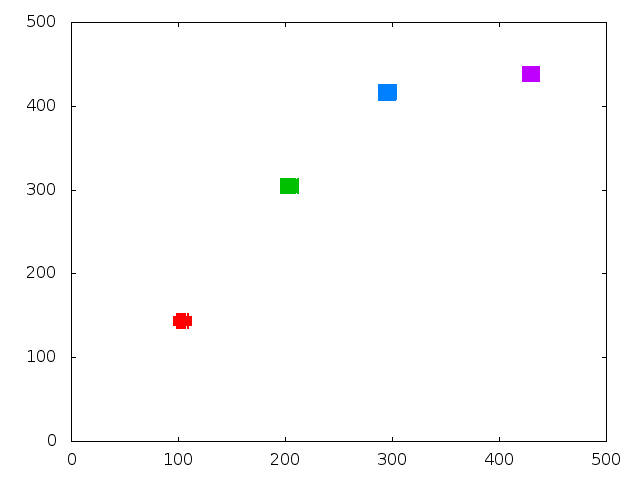
\includegraphics[width=5cm,height=5cm]{Trial1-0.png}
    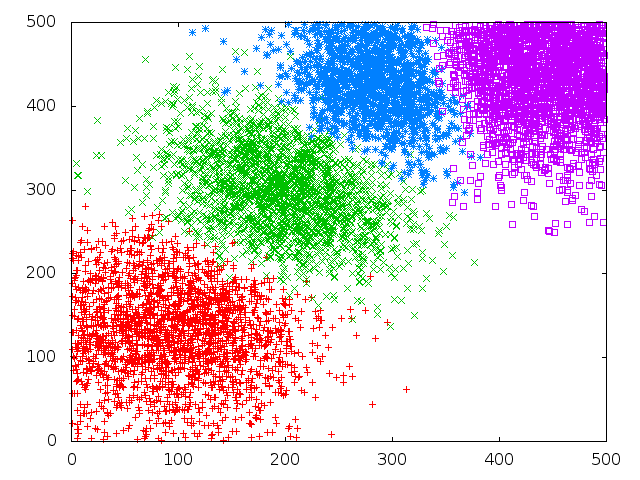
\includegraphics[width=5cm,height=5cm]{Trial1-5000.png}
    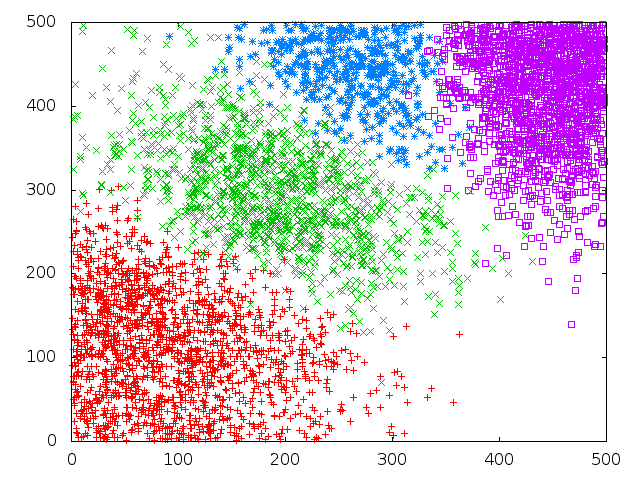
\includegraphics[width=5cm,height=5cm]{Trial1-10000.png}
    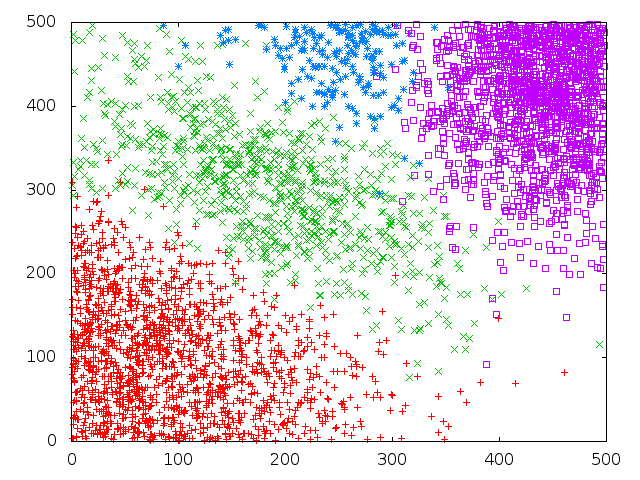
\includegraphics[width=5cm,height=5cm]{Trial1-15000.png}
    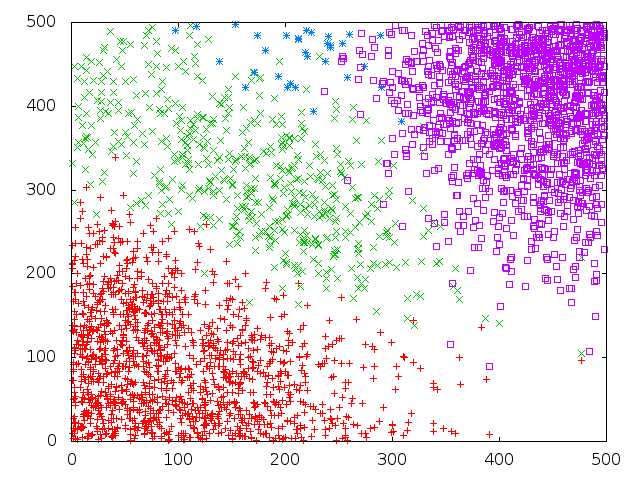
\includegraphics[width=5cm,height=5cm]{Trial1-20000.png}
    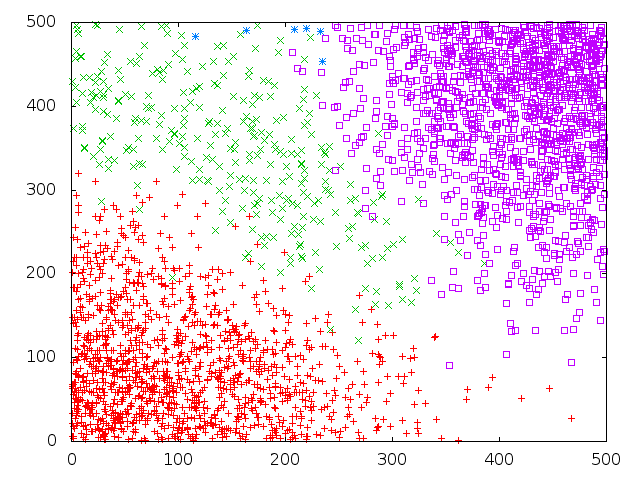
\includegraphics[width=5cm,height=5cm]{Trial1-25000.png}
    \caption{Results from first interesting trial}
\end{figure}

\begin{figure}
\centering
    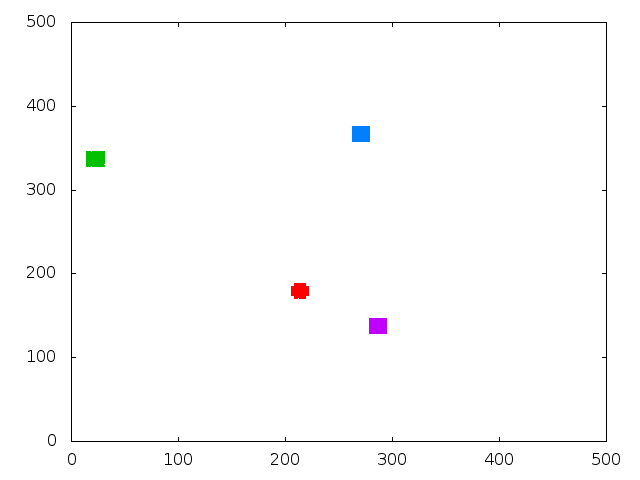
\includegraphics[width=5cm,height=5cm]{Trial2-0.png}
    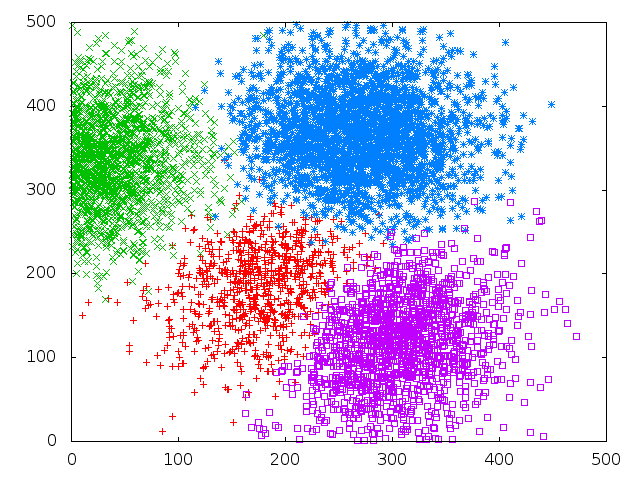
\includegraphics[width=5cm,height=5cm]{Trial2-5000.png}
    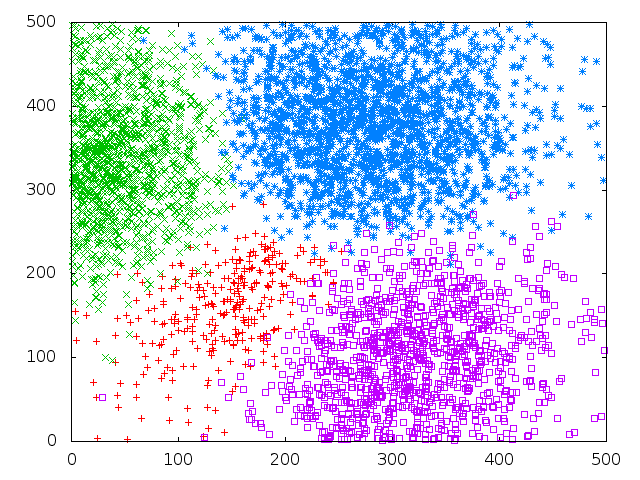
\includegraphics[width=5cm,height=5cm]{Trial2-10000.png}
    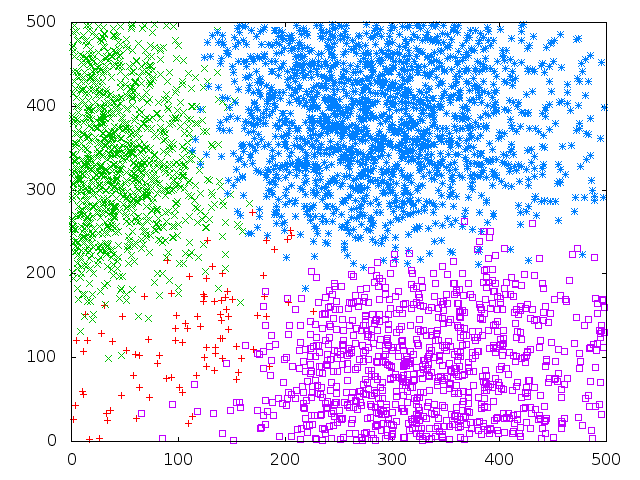
\includegraphics[width=5cm,height=5cm]{Trial2-15000.png}
    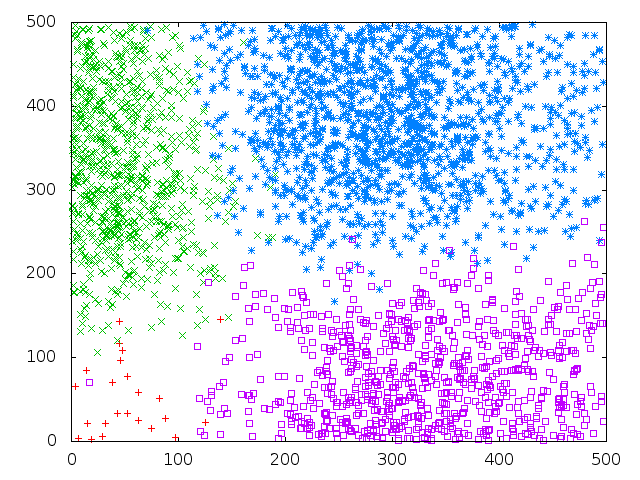
\includegraphics[width=5cm,height=5cm]{Trial2-20000.png}
    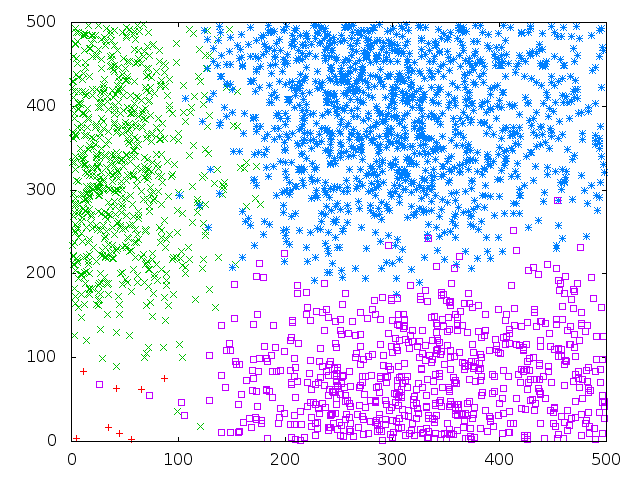
\includegraphics[width=5cm,height=5cm]{Trial2-25000.png}
    \caption{Results from second interesting trial}
\end{figure}

Note that, with the lack of a connected interface, these results depended on values
that were either set randomly or determined beforehand. In the interest of the
project, Jaysen did not devote his time to gathering data on this algorithm,
instead working closely with Paul in an attempt to get the interface functioning.\\
Therefore, these results are unfortunately far from a comprehensive analysis of
each of the properties of the agents.

There are some things that are noteworthy in these results, however. It appears
that a species' odds of survival are highly dependent on proximity to other species
-- note in the first trial that blue is the least advantaged in this situation, as
it is equidistant from green and purple and stuck between them. The others either
have further distance from some neighbors, or fewer neighbors. The advantage of
fewer neighbors is evident in the progress of red and purple, as their populations
boom.

In the second trial, it's worth noting that red had a very high predatory instinct,
which means that it sought out other species -- meanwhile, the others had a
relatively low predatory instinct, so they tried to avoid others. This worked to
the advantage of the ones that tried to avoid other species.

\subsection{The Client}
The important part of the client that needed to be tested was the EA. In trying to write the EA some test functionality was written to give a general sense of how things were evolving over time. The basic premise is to grab the species stats after every generation and store them, then display them all as a value over time plot using matplotlib. An example graph can be seen in Figure~\ref{ea_results}

\begin{figure}
\centering
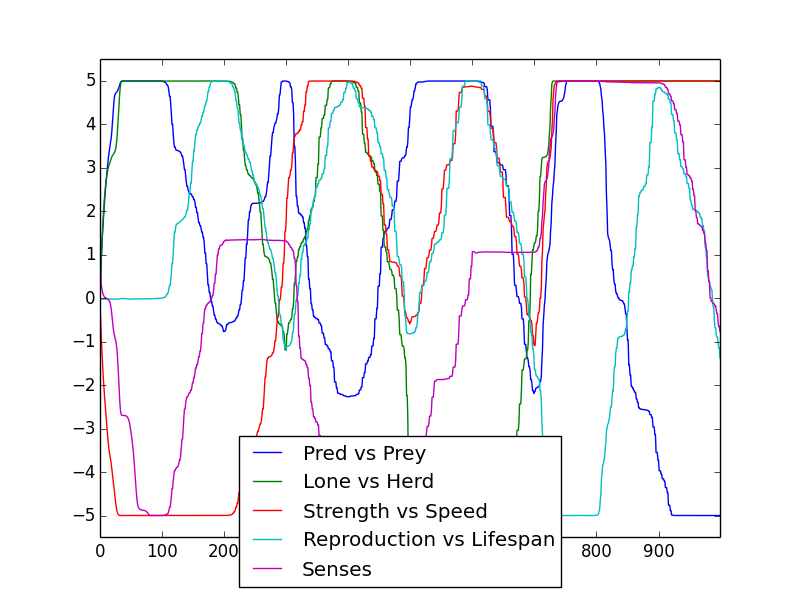
\includegraphics[width=\textwidth]{ea_results}
\caption{An example of the different traits evolving over time. Note: every 100 iterations the focus values were randomly changed.}
\end{figure}


% ~~~~~

\appendix

% Code
% !TEX root = FinalProject.tex

\chapter{Code}

\section{The Server}
\lstinputlisting[language=C++]{../Server/ServerEngine.cpp}

\section{The Client}
\lstinputlisting[language=Python]{../App/Client/Population.py}


\end{document}
